\section{Tests}

In den vorherigen Abschnitten haben wir die Funktionsweise des Brokers erläutert, den modularen Vorschlag als Python-Service implementiert, sowie Hyrise-R zum Cloud-Betrieb vorbereitet. Auf dem virtualisierten OpenStack-Testbed soll nun die Funktionsweise des Gesamtsystems geprüft werden: Zwei Hyrise-R-Cluster laufen über zwei Clouds verteilt und werden dynamisch skaliert, siehe \autoref{fig:hyrise-r-deployment}.

\begin{figure}[ht]
	%\begin{wrapfigure}{O}{0.3\textwidth}
	\centering
	%	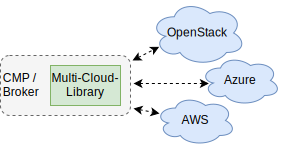
\includegraphics[width=0.48\textwidth]{images/multi-cloud-library.pdf}
	\def\svgwidth{0.75\textwidth}
	{\footnotesize \textsf{
			\includesvg{images/hyrise-r-deployment}}}
	\caption{Testarchitektur mit zwei Hyrise-R-Clustern, verteilt auf eine Public- und eine Private-Cloud. Cluster \emph{B} nutzt AWS, um unkritische Daten kostengünstig auszulagern. Orchestriert werden beide Services durch die selbst entwickelte Cloud-Management-Plattform aus der Private-Cloud heraus -- die CMP harmonisiert Provider- und Infrastrukturgefälle.}	
	\label{fig:hyrise-r-deployment}
	%\end{wrapfigure}
\end{figure}

Wir starten Hyrise-R immer als Cluster aus Dispatcher, Master und einer per SLO-Template bestimmten Anzahl an Replicas. Anschließend skalieren wir den Cluster dynamisch nach Leistungsanforderungen und SLO-Bedingungen. Das Re-deployment anhand von veränderter Umgebung ist eingeschränkt: Hyrise-R unterstützt keine Live-Migration. Einzig die Replicas lassen sich ohne Probleme an- und abmelden -- für Tests des Cloud-Burstings, also dem Abfangen erhöhter Last durch weitere Instanzen, ist das kein Problem: Entweder der Broker sucht eine passende Infrastruktur und startet einen neuen Hyrise-R-Replica-Knoten, oder er fährt einen Knoten herunter und meldet ihn ab. Die Tests sind rein qualitativ und decken folgende Fälle ab:

\begin{enumerate}
	\item Betrieb über Cloud-Grenzen hinweg
	\item Betrieb auf heterogener Infrastruktur
	\item Skalieren nach Leistungsanforderungen
	\item Skalieren nach weiteren SLOs und Nutzeranforderungen
\end{enumerate}

\todo{Tabelle der Testfälle}

In einem funktionsfähigen Hyrise-R-Cluster empfängt der Dispatcher alle Anfragen. Jede Anfrage mit Schreibanteil leitet er an den Master-Knoten. Hier wird die Anfrage bearbeitet, in das Log geschrieben und anschließend mit allen Replicas synchronisiert. Enthält eine Anfrage nur Leseanteile, verteilt der Dispatcher sie an einen beliebigen Knoten. Frühere Arbeiten bewerteten an dieser Stelle die Anfrageperformance und den Synchronisationsoverhead. Beide Metriken sind jedoch stark abhängig von der Performance der Cloud-Infrastruktur und Netzwerkverbindungen.

Als Metrik zur Bewertung des Brokerings gilt -- neben Einhaltung der SLOs -- die volle Funktionsfähigkeit des Clusters. Eine Beispieldatenbank ist bereits in den Images enthalten. Alle Anfragen haben ausschließlich lesende Anteile, die Tabelle wird nicht durch Schreibanfragen verändert und muss deshalb nicht synchronisiert werden. Gemessen wird also nicht die Synchronisationszeit der Hyrise-R-Lösung, sondern die Skalierungsfähigkeiten der verwendeten Cloud-Lösungen und Orchestrierungstechniken.

Die Hyrise-HTTP-Schnittstelle empfängt Anfragen im JSON-Format. Die minimale Anfrage \emph{NoOp} startet keine Datenbankoperation, durchläuft aber alle Datenbankkomponenten von HTTP-Handling über Parser bis Ausführungseinheit. Als erster Funktionstest würde diese Anfrage genügen. Wir möchten allerdings den gesamten Cluster testen, und nutzen daher eine echte, hinreichend komplexe Anfrage. Deren Bearbeitung benötigt genug Zeit, damit der Dispatcher sie auf alle Knoten aufteilen kann. Den vorhandenen Python-Code überarbeiten und parallelisieren wir. Die Anzahl der Knoten lässt eine bestimmte Performance erwarten -- für einen gültigen Test muss die Anzahl der Anfragen mindestens der Anzahl Knoten entsprechen:

\begin{minted}{python3}
queries = [(host, port, query)] * num_nodes
start_time = time.time()
with multiprocessing.dummy.Pool(num_threads) as pool:
	pool.starmap(query_hyrise, queries)
queries_second = num_nodes / (time.time() - start_time)
\end{minted}

Um sowohl OLTP- als auch OLAP-Fähigkeiten der In-Memory-Datenbank zu überprüfen, nutzen vorherige Arbeiten \cite{ssiclops:d42:experiments-measurements} den CH-benCHmark der TU München \cite{cole:2011:db-benchmark}. Dieser ist eine Mischung aus Transaktions- und Analysebenchmark, angelehnt an den hybriden Einsatz aktueller Datenbanksysteme in Unternehmen: Die gleichen Tabellen eines einzigen Datenbanksystems erfüllen alle Aufgaben des täglichen Geschäfts und liefern gleichzeitig umfassende Analysen. Trotzdem bleibt die Vergleichbarkeit des Benchmarks mit klassischen, getrennten Systemen.

Die Beispieldatenbank enthält eine Auftragshistorie mit knapp 300\,000 Datensätzen. Jede Zeile besteht aus sieben zufälligen Integer-, zwei String- und einem Float-Wert. So ergibt sich eine Rohgröße von 21,3\,MB. Die folgende Beispielanfrage\footnote{\url{https://db.in.tum.de/research/projects/CHbenCHmark/}} zeigt alle Bestellungen eines bestimmten Zeitraumes, sowie Summe, Gesamt- und Durchschnittswert aller enthaltenen Posten. Sie dient uns als \emph{Smoke-Test} -- liefert der Hyrise-R-Cluster eine valide Antwort im vorgegebenen Zeitrahmen, ist die generelle Funktionsfähigkeit gegeben, und das Deployment erfolgreich abgeschlossen:

\begin{minted}{sql}
SELECT ol_number,
       SUM(ol_quantity) AS sum_qty,
       SUM(ol_amount)   AS sum_amount,
       AVG(ol_quantity) AS avg_qty,
       AVG(ol_amount)   AS avg_amount,
       COUNT(*)         AS count_order
FROM orderline 
WHERE ol_delivery_d > '2007-01-02 00:00:00.000000' 
GROUP BY ol_number
ORDER BY ol_number
\end{minted}

Konkreter Test, SLOs: Verlinken aus vorherigem Abschnitt. 